\section{An Overview of \sys}
\label{sec:overview}
%!TEX root = ../../main.tex
\begin{figure}[t]
    \centering 
    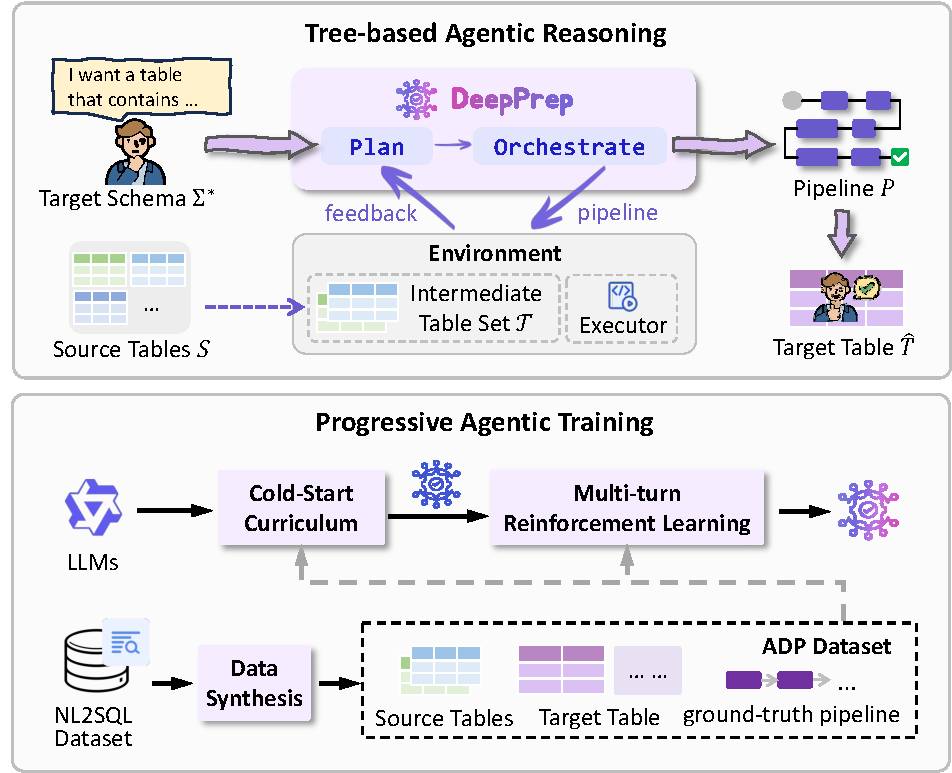
\includegraphics[width=0.9\columnwidth]{figures/fig/framework_overview.pdf}
   \vspace{-1em}
    \caption{An overview of \sys.
    }
    \label{fig:framework_overview}
   \vspace{-1em}
\end{figure}

\sys employs an agentic framework to autonomously orchestrate data preparation pipelines, as illustrated in Figure~\ref{fig:framework_overview}. Given a set of source tables $\mathcal{S}$ and a target schema $\Sigma^{\ast}$, \sys iteratively interacts with an \emph{environment} that executes data transformations and provides feedback.
%
The environment maintains an execution state represented by a set of intermediate tables, initialized with the source tables $\mathcal{S}$. Operator instances are executed within the environment through concrete execution backends (\eg a Python interpreter), which apply transformations to the current state and produce updated tables along with execution feedback.
%
Given the target schema $\Sigma^{\ast}$, \sys interacts with the environment through an iterative process that alternates among the \emph{planning}, \emph{orchestration}, and \emph{execution} steps, as described below.
%
\begin{itemize}[leftmargin=*]
    \item In the \emph{planning} step, the agent observes the current execution state and synthesizes a high-level textual plan that outlines how to transform the existing tables toward the target schema. 
    \item In the \emph{orchestration} step, \sys translates this plan into an executable pipeline by selecting appropriate operator types and instantiating them with specific parameters. 
    \item In the \emph{execution} step, the orchestrated pipeline is submitted to the environment, which executes the operators, updates its internal state with newly generated intermediate tables, and returns execution feedback, such as sample outputs or error traces.
\end{itemize}
%
Through iterative interaction with execution feedback, \sys progressively refines planning and orchestration decisions and converges to a pipeline that produces a desired target table.


%\sys employs an agentic framework to autonomously construct data preparation pipelines, as illustrated in Figure~\ref{fig:framework_overview}.
%Given a set of source tables $\mathcal{S}$ and a target schema $\Sigma^\ast$, \sys iteratively interactive with an \emph{Environment}. 
%The environment maintains the intermediate table set (initialized with source tables $\mathcal{S}$) and provides an execution interface for operators. Given a target schema $\Sigma^\ast$, \sys iteratively interacts with this environment through a feedback loop of \emph{planning}, \emph{orchestration}, and \emph{execution}.
% alternates between \emph{planning}, \emph{orchestration}, and \emph{execution}.
%In the \emph{planning phase}, the agent observes the current state of the environment and synthesizes a high-level textual plan to align the existing tables with $\Sigma^\ast$.
%In the \emph{orchestration phase}, \sys translates this plan into an executable pipeline by generating appropriate operators with specific parameters.
%Subsequently, in the \emph{execution phase}, the orchestrated pipeline is submitted to the environment. The environment executes the operators, updates its internal state to include the resulting intermediate tables, and returns execution feedbacks (\eg sample data of generated table or error traces) to the agent.
% If successful, the environment is updated with the resulting intermediate tables; otherwise, the execution error is captured to inform subsequent iterations.
%Through this feedback loop, \sys progressively refines the environment state, converging to a pipeline that generates a target table satisfies the target schema.

\begin{example}
    Consider the ADP task shown in Figure~\ref{fig:introduction_example}. The environment is initialized with the source tables and target schema. 
    % At each iteration, \sys observes the current execution state, including serialized table contents and available schema information.
    %
    \begin{itemize}[leftmargin=*]
    \item To align the data with the target schema, the agent first generates a high-level textual plan, such as ``Clean table \textit{movies}...''. 
    \item Based on this plan, the orchestration step instantiates a pipeline, \ie a sequence of operators, \eg \texttt{Deduplicate(\ldots)} followed by \texttt{ValueTransform(\ldots)}. The orchestrated operators are then submitted to the environment for execution. 
    \item Upon execution, the environment applies the operators to the current state and returns execution feedback. Specifically, if execution is successful, the environment updates its state to include the cleaned movies table while retaining the original ratings and directors tables. Otherwise, execution errors are captured and propagated to the agent to revise subsequent decisions.
    \end{itemize}
    %
    The iterative process continues until the generated tables satisfy the target schema and quality requirements, at which point \sys terminates and outputs the final data preparation pipeline.
    %
    %Consider the ADP task in Figure~\ref{fig:introduction_example}. The environment is initialized with the source tables. \sys first observes the serialized table content and schema. To align with the target schema, it generates a high-level plan: ``Clean table \textit{movies} and then integrate with \textit{ratings}.'' Based on this, \sys orchestrates a sequence of operators, \eg \texttt{Deduplicate($\ldots$)} and \texttt{ValueTransform($\ldots$)}. These are submitted to the environment, which executes them and updates its internal state to contain the cleaned \textit{movies} table alongside the original \textit{ratings} and \textit{directors} for the next iteration.
\end{example}

To support the framework, we design two key components: \emph{Tree-Based Agentic Reasoning} and \emph{Progressive Agentic Training}.

\stitle{Tree-based Agentic Reasoning.}
The key challenge in agentic pipeline orchestration is supporting \emph{structured} exploration and backtracking under execution feedback. Specifically, pipeline construction involves interdependent operator decisions, where early choices may later prove suboptimal or infeasible. Linear agentic reasoning mechanisms such as ReAct~\cite{aksitov2023rest} and CoT~\cite{wang2024chain} follow a single decision trajectory and do not preserve alternative paths. Thus, once a candidate pipeline is executed, early errors can propagate to subsequent steps, and without a structured representation that retains historical states, recovery becomes difficult.

To address this challenge, we introduce a \emph{tree-based agentic reasoning} mechanism. Instead of committing to a single linear execution trajectory, \sys represents pipeline construction as a search tree, where each node corresponds to a planning state associated with a set of intermediate tables, and each edge represents applying a candidate operator pipeline. This tree structure preserves historical states and alternative construction paths, enabling systematic exploration and backtracking based on execution feedback.
Building on this tree representation, we further define LLM interaction patterns and decision logic over the tree, allowing the agent to reason about which branch to expand, revise, or abandon during pipeline construction. We detail this tree-based reasoning and interaction mechanism in Section~\ref{sec:tree_based_agentic_reasoning}.

\stitle{Progressive Agentic Training.}
The key challenge is how to effectively train LLMs for tree-based agentic reasoning.
A straightforward approach is to directly apply existing reinforcement learning methods to optimize the model using outcome-level rewards.
However, this setting poses two major difficulties.
First, \emph{reward sparsity}: data preparation pipelines often consist of long and interdependent operator sequences, and relying solely on final correctness makes it difficult for the model to learn structured exploration and non-local backtracking behaviors.
Second, \emph{data scarcity}: existing ADP datasets mainly involve simple transformations with short operator sequences~\cite{DBLP:journals/pvldb/LiHYWC23, lai2025auto}, providing insufficient supervision for learning multi-step reasoning that depends on execution feedback.

To address reward sparsity, we first introduce a Cold-Start Curriculum that initializes the model with basic knowledge of data preparation operators and the tree-based agentic reasoning procedure.
Next, we apply multi-turn reinforcement learning with a Hybrid Reward mechanism that combines outcome-level signals with process-level feedback.
To alleviate data scarcity, we develop a data synthesis approach that generates complex ADP tasks grounded in meaningful analytical transformations, while injecting diverse data quality issues without breaking the intended transformation logic.
We detail our agentic training strategy in Section~\ref{sec:agentic_training_framework}.

%The key challenge in agentic training stems from the complexity of tree-based agentic reasoning. 
%Unlike linear agentic reasoning, the agent must learn to operate over a {branching search structure}, including how to expand promising branches, revise earlier decisions, and backtrack based on execution feedback.
%This complexity imposes two fundamental obstacles:
%(1) \textit{Reward Sparsity}. The inherent complexity above makes it difficult for foundation LLMs to complete ADP tasks successfully during the early stages of training. This brings a lack of positive reinforcement signals, which can hinder or even collapse the entire agentic training process.
%(2) \textit{Data Scarcity}. Current ADP datasets, either focus on isolated sub-tasks~\cite{DBLP:journals/pvldb/LiHYWC23} or only involve fewer than 2 operators~\cite{lai2025auto}. Such simple ADP tasks, fail to train an agent of agentic tree-based reasoning, since they can be solved within one-shot generation.

%To address the reward sparsity, we propose a \emph{Progressive Agentic Training} strategy, which decomposes the learning process into multiple stages. Instead of directly forcing the model to learn the agentic tree-based reasoning in complex ADP scenarios. This step-by-step strategy enables the model to evolve from memorizing the operator syntax and reasoning protocol. In addition, we accept the partial-correct reasoning trajectories by calculating the ``similarity'' between the generated table and target table.
%To address the data scarcity, we collect data from NL2SQL datasets to get the source tables and target table pair. These table pairs implies data requirements in real life and complex data mapping, which can serve as the high quality data source in our training framework. Moreover, to further enhance diversity to ensure the generalization capability of agent trained on the synthesized data, we inject dirty data to the clean and relational source tables with a Reverse Operator Injection module.
%We detail our agentic training strategy in Section~\ref{sec:agentic_training_framework}.